\chapter{Estado del arte} \label{ich:estado_arte}

Procedemos a realizar un estudio del estado del arte para el problema que buscamos resolver. Consultaremos los mejores resultados para la tarea de \textit{retrieval } en reconocimiento facial invariante a la edad sobre el conjunto de datos \textit{FG-Net}. Esto porque, como ya hemos comentado en \customref{isubsubs:fgnet_inconvenientes}, y motivados por el trabajo de \cite{informatica:best_fgnet_model}, nuestro enfoque va a ser el siguiente: realizar un entrenamiento sobre el conjunto de datos \textit{CACD}, y usar \textit{FG-Net} para validar nuestro modelo.

No es de interés estudiar los resultados de modelos sobre \textit{CACD}, porque estamos usando dicho conjunto para entrenar. Además, la mayoría de trabajos que estudiaremos más adelante, usan un \textit{dataset} de tamaño considerable para entrenar, y evalúan sobre \textit{FG-Net}. Su \textit{dataset} de entrenamiento no tiene por qué ser \textit{CACD}. Con esto queda claro que lo que realmente nos interesa son los resultados sobre \textit{FG-Net}.

\section{Interés del área de estudio} \label{isec:interesareaestudio}

Empecemos viendo el interés de este área de estudio. Para ello podemos realizar una búsqueda en \textit{SCOPUS}, buscando trabajos sobre \textit{AIFR}, filtrando el área de estudio al de las ciencias de la computación. Esto produce los siguientes \textit{keywords}:

\begin{lstlisting}[caption=\textit{Keywords usados para la búsqueda en \textit{SCOPUS}}, label=code:scopus_search]
    TITLE-ABS-KEY ( age  AND invariant  AND face  AND recognition )  AND  ( LIMIT-TO ( SUBJAREA ,  "COMP" ) )
\end{lstlisting}

Con dichos \textit{keywords} obtenemos la siguiente gráfica:

\begin{figure}[H]
    \centering
    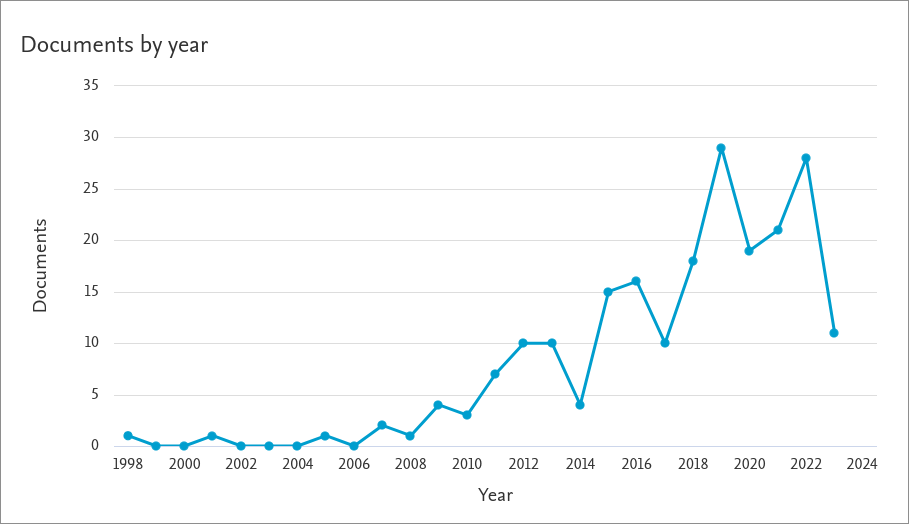
\includegraphics[width=0.6\textwidth]{informatica/scopus_search_histogram}
    \caption{Resultados de la búsqueda en \textit{SCOPUS} usando los \textit{keywords} \customref{code:scopus_search}}
\end{figure}

Vemos que, a partir de 2012 (momento que coincide con la aparición de \textit{AlexNet} y que da paso a la popularidad de redes convolucionales profundas en el campo de la imagen) este área de estudio gana bastante popularidad. Sin tener en cuenta el último año (pues, en el momento de la consulta, sigue en curso y está lejos de acabar), no vemos que la tendencia siga al alza, pudiendo llegar a pensar que la popularidad de este campo se está estancando. Aunque habría que tener en cuenta condiciones externas, como la pandemia de \textit{COVID}, que podrían explicar la bajada notable en los años 2020 y 2021.

Veamos también la popularidad de la técnica \textit{triplet loss}, pues estamos proponiendo una mejora sobre esta. Los \textit{keywords} usados fueron:


\begin{lstlisting}[caption=\textit{Keywords usados para la búsqueda en \textit{SCOPUS} para consultar la popularidad del \textit{triplet loss}}, label=code:scopus_search_tripletloss]
    TITLE-ABS-KEY ( triplet  AND loss )  AND  ( LIMIT-TO ( SUBJAREA ,  "COMP" ) )
\end{lstlisting}

La búsqueda con estos \textit{keywords} produce la siguiente gráfica:

\begin{figure}[H]
    \centering
    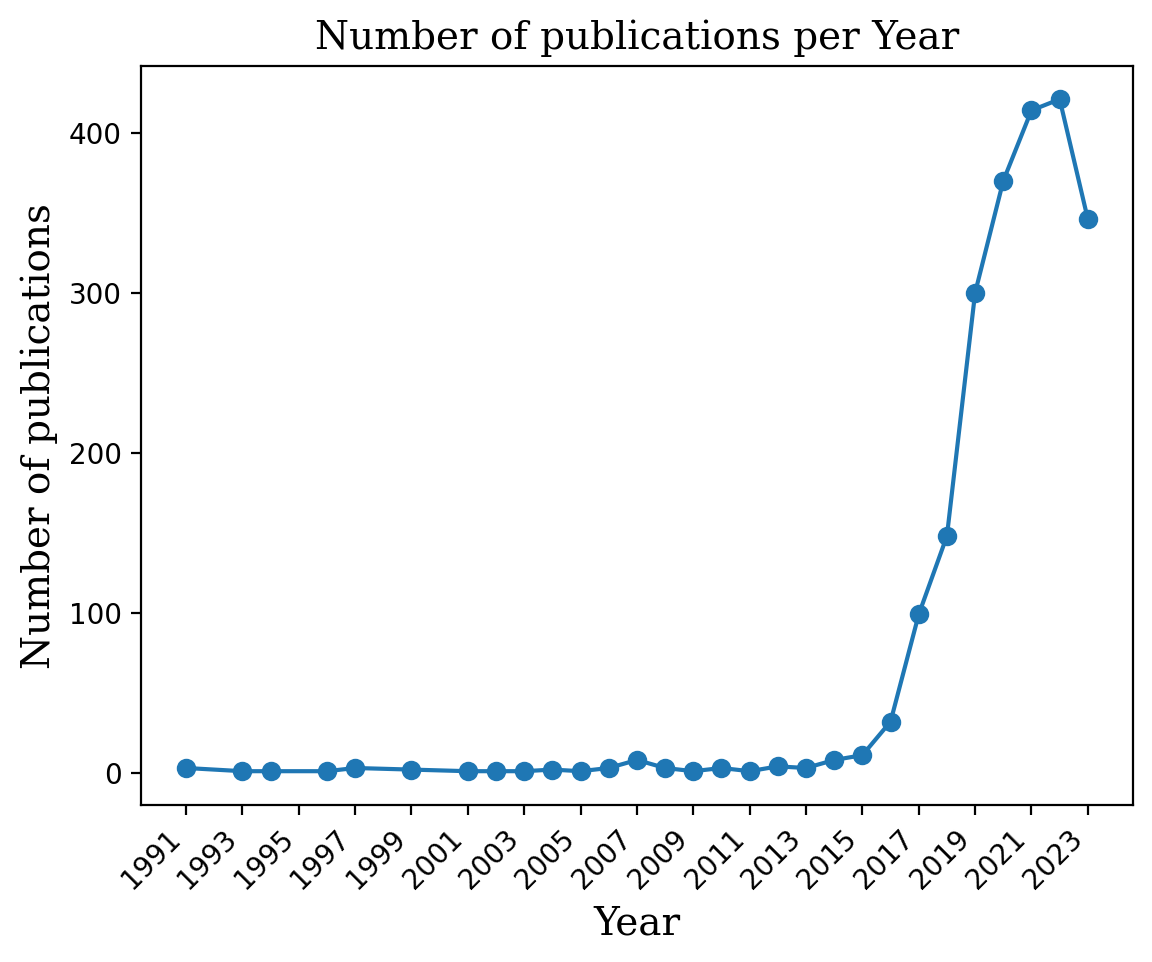
\includegraphics[width=0.6\textwidth]{informatica/scopus_search_tripletloss}
    \caption{Resultados de la búsqueda en \textit{SCOPUS} usando los \textit{keywords} \customref{code:scopus_search_tripletloss}}
\end{figure}

Vemos que entre 2017 y 2018 esta técnica da un grandísimo salto en popularidad. Sin embargo, en los dos últimos años la popularidad ha caído en picado, y aunque todavía no haya pasado el tiempo suficiente para observar el progreso de dicha tendencia, la caída en el último año es demasiado grande, y pensamos que la tendencia va a seguir a la baja.

Por otro lado, estamos usando nuevas técnicas para computar \textit{triplet loss}. Dichas técnicas fueron introducidas en \cite{informatica:principal}. En dicho trabajo se intenta resolver una tarea de re-identificación, que difiere de nuestra tarea de \textit{retrieval} para reconocimiento facial invariante a la edad. Por lo tanto, buscamos trabajos que hayan aplicado \textit{triplet loss} en el campo del \textit{AIFR}. Aplicamos la siguiente búsqueda:

\begin{lstlisting}[caption=Keywords usandos para la búsqueda de trabajos que combinen \textit{AIFR} y \textit{triplet loss} en \textit{SCOPUS}, label=code:scopus_search_especifico]
    TITLE-ABS-KEY ( age AND invariant AND face AND recognition, AND triplet AND loss )  AND  ( LIMIT-TO ( SUBJAREA ,  "COMP" ) )
\end{lstlisting}

La búsqueda determinada por \customref{code:scopus_search_especifico} no produce ningún resultado. \textbf{No hay publicado ningún trabajo que aplique \textit{triplet loss} al campo del \textit{AIFR}}. Y esto, sin considerar que nuestro trabajo introduce nuevas técnicas que mejoran el uso del \textit{triplet loss} clásico, desarrollado en \customref{isec:triplet_loss}.

Así que, cuando veamos en \customref{ich:conclusiones} que no obtenemos buenos resultados, tendremos que \textbf{justificar el por qué basándonos únicamente en el trabajo presente}, puesto que \textbf{ningún trabajo ha intentado resolver una tarea de \textit{AIFR} usando \textit{triplet loss}}.

\section{Mejores modelos de \textit{retrieval} para el \textit{dataset} \textit{FG-Net}}

En esta sección vamos a introducir los mejores modelos que resuelven una tarea de \textit{retrieval} sobre el \textit{dataset} \textit{FG-Net}. Como ya hemos visto en \customref{isec:interesareaestudio}, ninguno de estos modelos usará \textit{triplet loss}. Por lo tanto, será complicado justificar las diferencias en los resultados obtenidos.

\subsection{When Age-Invariant Face Recognition Meets Face Age Synthesis: A Multi-Task Learning Framework} \label{isubs:mtl_face}

El trabajo realizado en \cite{informatica:best_fgnet_model} propone el modelo \textit{MTLFace}. Dicho modelo se construye optimizando una función multiobjetivo.

Para ello, se da un primer paso que consiste en la obtención de dos \textit{features} incorreladas: edad e identidad. Para ello, usan una arquitectura basada en mecanismos de atención. A partir de esto, se realiza el aprendizaje de la función multiobjetivo. Por un lado, se debe resolver la tarea de, dada una imagen de una persona, estimar su edad. Y por otro lado, el del reconocimiento facial: dadas dos imágenes de la misma persona (resp. dos personas distintas) identificar que son la misma persona (resp. identificar que no son la misma persona).

Para obtener buenos resultados sobre \textit{FG-Net}, proponen la creación de un nuevo \textit{dataset}, que combina varios \textit{datasets} en uno.

Además, usan modelos generativos adversarios \textit{GANs} para, dada la imagen de una persona, y una edad objetivo, generar una posible imagen de esa persona a la edad dada. Esto es utilizado en el proceso de aprendizaje. La siguiente figura muestra dicho proceso sintético:

\begin{figure}[H]
    \centering
    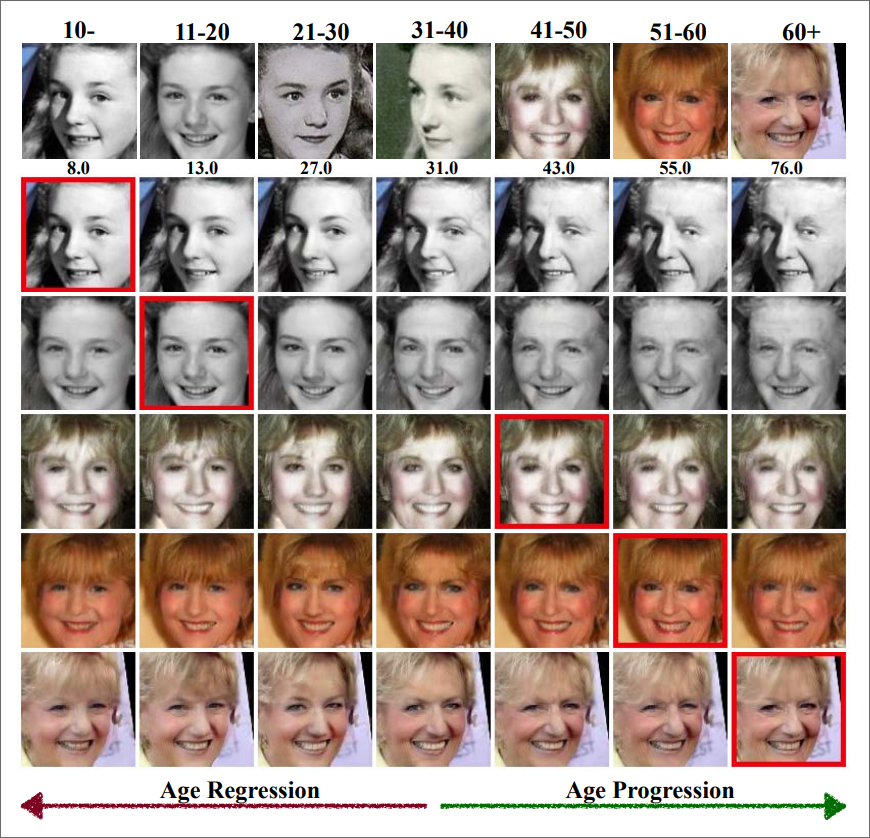
\includegraphics[width=0.6\textwidth]{informatica/mtlface_generativo}
    \caption{Ejemplo de los resultados del modelo generativo usado en el entrenamiento. La primera fila muestra imágenes reales de una persona en distintas etapas de su vida. Las siguientes filas son imágenes generadas cuando se da como entrada la imagen marcada en rojo. Imagen extraída de \cite{informatica:best_fgnet_model}}
\end{figure}

Este trabajo obtiene para la métrica \textit{Rank@1} un valor de 94.78\% \footnote{En dicho trabajo, se refieren a dicha métrica como \textit{leave one out}. Dicho nombre está justificado por el proceso que supone el cálculo de la métrica, como hemos explicado previamente. El otro protocolo, \textit{MF1}, que supone evaluar añadiendo un conjunto de imágenes distractoras, no lo consideramos pues no lo hemos implementado }

\subsection{Decorrelated Adversarial Learning for Age-Invariant Face Recognition}

El trabajo realizado en \cite{informatica:dal} propone eliminar los factores asociados a la edad en la representación que su modelo aprende. En la misma línea que \customref{isubs:mtl_face}, se buscan aprender dos \textit{features} incorreladas, una asociada a la edad, y otra asociada a la identidad. Se propone el algoritmo de aprendizaje \textit{Decorrelated Adversarial Learning} o \textit{DAL}. Se emplea un módulo \textit{Canonical Mapping Module} con el objetivo de buscar la máxima correlación entre los pares de \textit{features} generados por la red neuronal. Por lo tanto, actuará como discriminador en un escenario adversario. La red se entrena para que la correlación de dichos pares sea lo menor posible.

La siguiente imagen servirá para entender mejor la descomposición en dos \textit{features} incorreladas:

\begin{figure}[H]
    \centering
    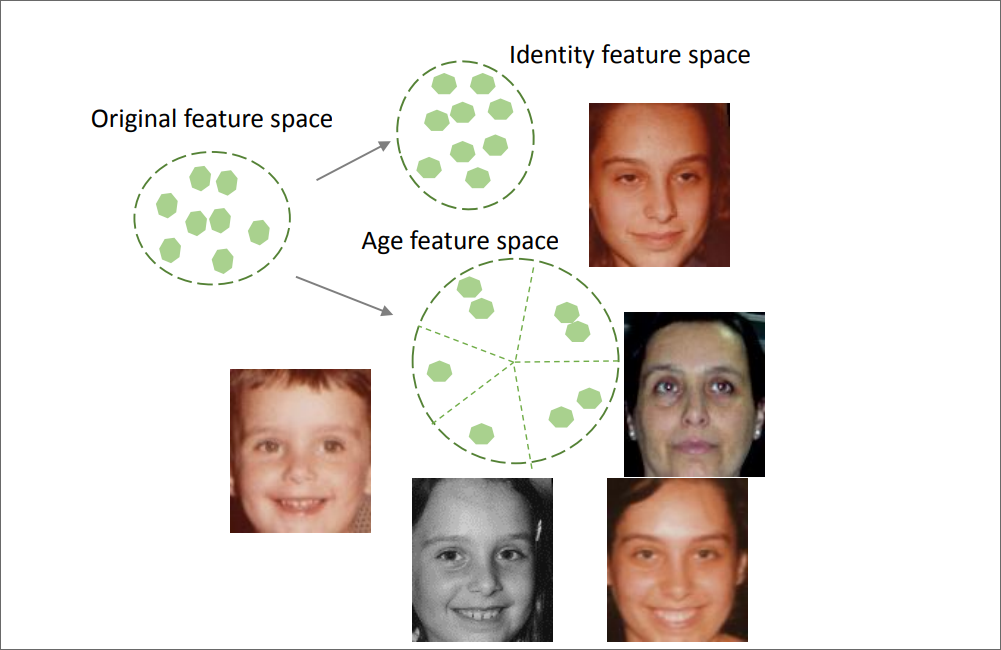
\includegraphics[width=0.6\textwidth]{informatica/dal_descomposicion}
    \caption{Ejemplo de cómo estamos descomponiendo la información en dos componentes: una de edad y otra de identidad. Estas imágenes muestran como, fijada la componente de identidad, podemos variar la componente de edad. Imagen extraída de \cite{informatica:dal}}
\end{figure}

Se obtiene un valor de 94.5\% para \textit{Rank@1}.

\subsection{Look Across Elapse: Disentangled Representation Learning and Photorealistic Cross-Age Face Synthesis for Age-Invariant Face Recognition}

El trabajo desarrollado en \cite{informatica:aim} propone, de nuevo, extraer conjuntamente \textit{features} sobre la edad e identidad de las imágenes, introduciendo el modelo \textit{Age Invariant Model} o \textit{AIM}.

Y de nuevo, realizan una tarea de síntesis y discriminación adversaria para el aprendizaje del modelo. En dicho proceso, se obtiene un generador fotorealista. Esto es, dada una imagen de entrada y una edad objetivo, el generador es capaz de crear una posible imagen de la persona con esa edad, de una calidad muy alta.

Además, construyen un nuevo \textit{dataset} para ser usado como \textit{benchmark}, el \textit{dataset} \textit{Cross-Age Face Recognition} o \textit{CAFR}.

\begin{figure}[H]
    \centering
    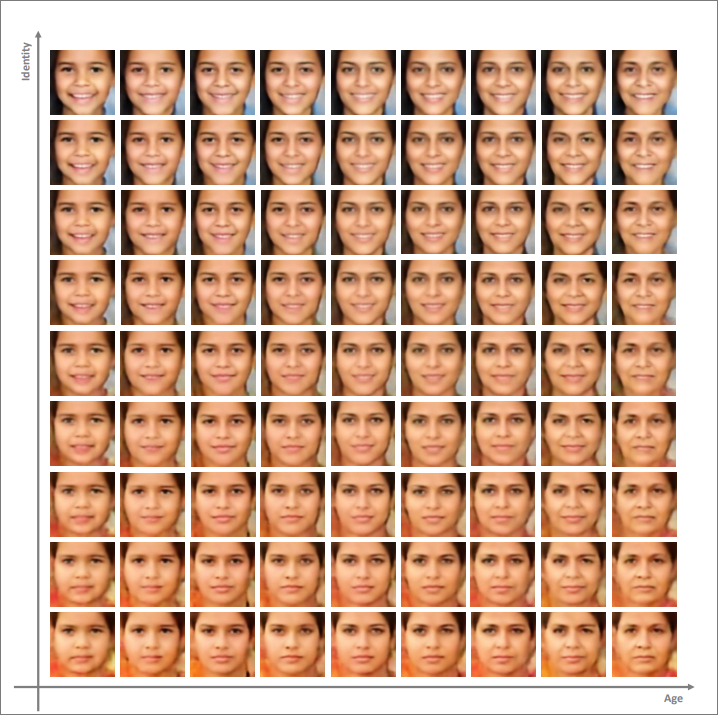
\includegraphics[width=0.6\textwidth]{informatica/aim_manifold}
    \caption{Espacio aprendido, continuo sobre las \textit{features} de edad (eje horizontal) e identidad (eje vertical). Imagen extraída de \cite{informatica:aim}}
\end{figure}

En dicha figura se puede observar lo que acabamos de comentar: el generador obtenido es de una grandísima calidad. Y podemos variar de forma continua la identidad o la edad de la imagen que queremos generar.

Se obtiene un valor de 93.20\% para \textit{Rank@1}

\subsection{Comparativa de todos los trabajos estudiados}

Mostramos ahora, de forma resumida, una comparativa de los resultados obtenidos por los trabajos que acabamos de estudiar:

\begin{table}[H]
\centering
\begin{tabular}{|l|l|}
    \hline
    Modelo & \textit{Rank@1} \\
    \hline

    \textbf{\textit{MTLFace}} & \textbf{94.78} \\
    \textit{DAL} & 94.5 \\
    \textit{AIM} & 93.20 \\
    \hline

\end{tabular}
\caption{Resultados de los principales modelos estudiados del estado del arte sobre el \textit{dataset} \textit{FG-Net}. La métrica \textit{Rank@1} también aparece referenciada en estos trabajos como \textit{leave one out}}
\end{table}

Y ahora, usando la comparativa que aparece en \cite{informatica:best_fgnet_model}, mostramos los resultados de otros modelos, cuyos trabajos no hemos estudiado:

\begin{table}[H]
\centering
\begin{tabular}{|l|l|}
    \hline
    Modelo & \textit{Rank@1} \\
    \hline
    HFA & 69.00 \\
    MEFA & 76.20 \\
    CAN & 86.50 \\
    LF-CNN & 88.10 \\
    AIM & 93.20 \\
    DAL & 94.50 \\
    \textbf{MTLFace} & \textbf{94.78} \\
    \hline
\end{tabular}
\caption{Resultados de algunos modelos sobre el \textit{dataset} \textit{FG-Net}. Datos extraídos de \cite{informatica:best_fgnet_model}}
\end{table}

\section{Conclusiones}

En base a el estudio realizado sobre otros trabajos relacionados, sacamos las siguientes \textbf{conclusiones}:

\begin{itemize}
    \item \textbf{No existen trabajos previos que empleen \textit{triplet loss} para resolver una tarea de \textit{AIFR}}. Por lo tanto, no podremos contrastar los resultados obtenidos con modelos que operen de una forma parecida
    \item \textbf{Los mejores modelos sobre \textit{FG-Net} emplean técnicas mucho más avanzadas} que las presentadas en este trabajo. El aprendizaje de dos \textbf{\textit{features} incorreladas}, una para la edad y otra para la identidad es el factor común en los modelos que obtienen mejores resultados. Unos trabajos desarrollan este aprendizaje usando \textbf{modelos basados en mecanismos de atención} o esquemas \textbf{generativos adversarios}
    \item Por lo tanto, parece que nuestra propuesta no va a ser lo suficientemente potente como para obtener los resultados aquí mostrados. Sin embargo, sería realmente interesante obtener resultados competentes de un modo u otro, pues obtendríamos un modelo mucho más ligero a partir de un entrenamiento mucho más fácil de realizar, tanto por los recursos empleados como por las técnicas empleadas
\end{itemize}
